% This text is proprietary.
% It's a part of presentation made by myself.
% It may not used commercial.
% The noncommercial use such as private and study is free
% Sep. 2005 
% Author: Sascha Frank 
% University Freiburg 
% www.informatik.uni-freiburg.de/~frank/


\documentclass{beamer}
\begin{document}
\title{Hello, I'm VM, Dalvik VM!}   
\author{Dainius Jocas} 
\date{\today} 

\frame{\titlepage} 

%% plan:
%% - review af technical report
%% - and preparation for code review
%% - what properties dalvik VM has, and next time we'll how this is achieved in code
%% IDEA: to present code which is executed when the application is started
%% probably the dexopt module
%% inversion of control (template method) (dependency injection) -- try to find it in code
%% method by method what is happening when the application is starting. From activity
%% http://www.kandroid.org/online-pdk/guide/dalvik.html

\frame{\frametitle{Table of contents}\tableofcontents} 


\section{Introduction} 
\frame{\frametitle{What is a VM?} 
    A virtual machine (VM) is a software implemented abstraction of the underlying hardware, which is presented to the application layer of the system.
}

\frame{\frametitle{Dalvik and Android}
  \begin{figure}
  \center
  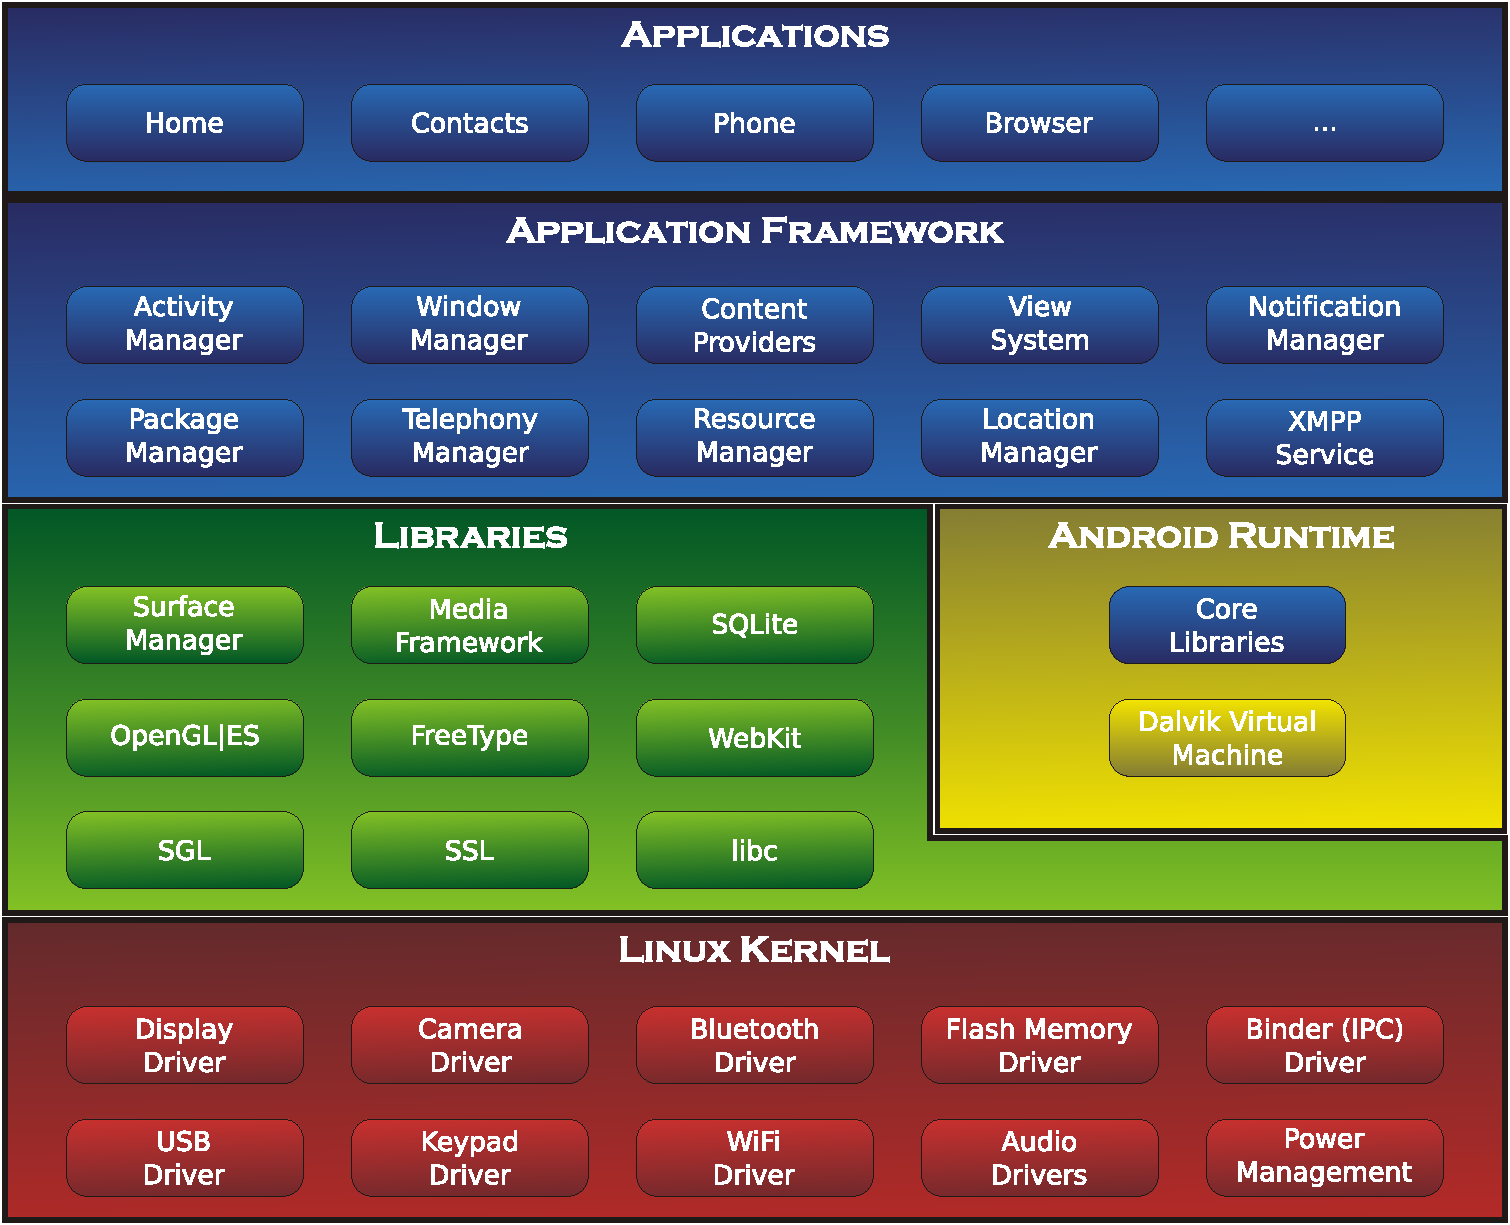
\includegraphics[width=0.8\textwidth]{./images/android_system_architecture.pdf}
\end{figure} 
%% Run-time system, software designed to support the execution of computer programs.
%% objdump (part of the GNU Binutils) is a program for displaying various information about object files
}

\frame{\frametitle{Some picture}
  \begin{figure}
  \center
  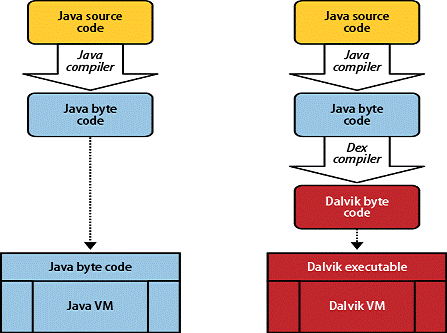
\includegraphics[width=0.8\textwidth]{./images/rVSX8.png}
\end{figure} 
%% Run-time system, software designed to support the execution of computer programs.
%% objdump (part of the GNU Binutils) is a program for displaying various information about object files
}

\frame{\frametitle{Dalvik VM}
  \textbf{Definition}: The Dalvik Virtual Machine is the heart of Android. It's a fast, just-in-time compiled, optimized bytecode virtual machine. Android applications are compiled to Dalvik bytecode and run on the Dalvik VM.
  
  What it means:
  \begin{itemize}
    \item fast?
    \item just-in-time compiled?
    \item optimized bytecode?
  \end{itemize}
}

\frame{\frametitle{Speed}
  \begin{itemize}
    \item .dex files are smaller in size compared to .jar files.
    \item Dalvik is a register based VM.
	\item .dex produced in that way, that they have a more dense encoding.
  \end{itemize}
  }

\frame{\frametitle{Just-in-time compilation}
  \begin{itemize}
    \item Just-in-time (JIT) compilation, also known as a dynamic translation, is a technique for improving the runtime performance of computer program based on byte code.	
    \item Translation of interpretable bytecode into an executable machine code.	
    \item Because Dalvik is register based VM, JIT compiler is simpler.
  \end{itemize}
}

\frame{\frametitle{Optimizations on bytecode}
  \begin{itemize}
    \item Constant pool references are replaced with pointers to internal data structures
    \item inlining of methods
    \item prune empty methods
    \item append pre-computed data
    \item ...
  \end{itemize}
}

\frame{\frametitle{Dalvik instructions}
  \begin{itemize}
    \item \textsc{01 12x 	move vA, vB}
    \item 16-bit instruction set.
    \item 226 instructions (during the optimization step new opcodes may appear).
    \item When used for bit values (such as integers and floating point numbers), registers are considered 32 bits wide. Adjacent register pairs are used for 64-bit values.
  \end{itemize}
}

\section{On the way to investigate Source Code}

\frame{\frametitle{Android source code. Numbers}
  \begin{itemize}
    \item Whole Android project: 279,843 items, totalling 7.0 GB
    \item Dalvik VM: 4,142 items, totalling 29.6 MB
    \item Dalvik VM is implemented in C, C++, Assembly, and Java
  \end{itemize}
}

\frame{\frametitle{Dalvik's Toolkit}
  \begin{itemize}
    \item dx -- the tool that takes in class files and reformulates them for consumption in the Dalvik VM.
    \item dexopt -- performs an abbreviated VM initialization, loads zero or more DEX files from the bootstrap class path, and then sets about verifying and optimizing whatever it can from the target DEX.
    \item dexdump -- tool is intended to mimic "objdump" - program for displaying various information about object files.
    \item dexdeps -- DEX external dependency dump
    \item ...
  \end{itemize}
}



%% https://blogs.oracle.com/jrose/entry/with_android_and_dalvik_at
\end{document}

